\section{Construction}

\subsection{Fixation des moteurs}
\begin{frame}
  \frametitle{Fixation des moteurs}
  \begin{columns}[c]
    \begin{column}[T]{.5\textwidth}
      \frametitle{Fixation}
      \begin{itemize}
        \item moteur visser sur la pièce en plastique
        \item pièce en plastique visser sur les articulation
        \item empreinte pour les écrous
        \item facile à assembler et désassembler
      \end{itemize}
    \end{column}
    \begin{column}[T]{.5\textwidth}  
      \begin{figure}
        			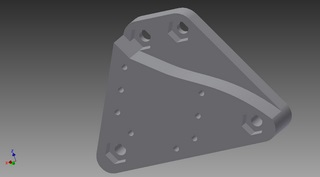
\includegraphics[width=5cm]{../img/part_middle_v1.jpg}
      \end{figure}
    \end{column}
  \end{columns}
\end{frame}

\subsection{Problème rencontré}
\begin{frame}
  \frametitle{Problème rencontré}
  \begin{itemize}
    \item pièce bottom 
      \begin{itemize}
        \item 1*AX12
        \item 2*AX12 
        \item 1*MX28
        \item raccourcissement des tubes
      \end{itemize}
    \item pièce top
      \begin{itemize}
        \item buté contre le plastique
        \item inversement des axe de rotation des moteur
      \end{itemize}
    \item pièce cou
      \begin{itemize}
        \item casse de la pièce
      \end{itemize}
  \end{itemize}
\end{frame}

\subsection{Contrôle des LED}
\begin{frame}
  \frametitle{Contrôle des LED}
  \begin{columns}[c]
    \begin{column}[T]{0.5\textwidth}
      \begin{itemize}
        \item arduino
        \item utilisation de transistor
        \item communication série pour changer de couleur
      \end{itemize}
    \end{column}
    \begin{column}[T]{0.5\textwidth}
      \begin{figure}
        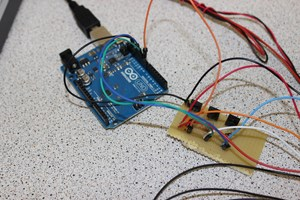
\includegraphics[width=5cm]{../img/arduino+transistorcard.JPG}
      \end{figure}
    \end{column}
  \end{columns}
\end{frame}
